\section{Education and Training}
\label{sec:education}
\subsection{\bf About the ACMS program}

The ACMS {\em (Applied and Computational Mathematical Sciences)} was
introduced in 1998 as a joint undergraduate program between the
departments of Applied Mathematics, Computer Science and Engineering,
Mathematics and Statistics, among others.

The ACMS program is structured into a {\em core}, totaling 43 credits,
and a set of options, or {\em tracks}. The same set of core courses is
required for all options (with some exceptions). Options are either
associated with a particular application domain (Biological and Life
Sciences, Mathematical Economics, Social and Behavioral Sciences,
Engineering and Physical Sciences) or with a particular area of
specialization in the mathematical sciences ({\em Discrete Math and
  Algorithms, Operations Research, Scientific Computing and Numerical
  Analysis, and Statistics}). 

It is the Statistics track of ACMS that we are aiming to
tranform. Currently, this track contains, in addition to the core
courses (43 credits), the following:
\\
{\bf Option Core (37 credits)}
\bits
    \item {\sc PHYS 121-2-3} (replaceable by other courses in application areas)
    \item {\sc STAT 302} Statistical Software and Its Applications (R course, irregularly offered, 2 credits)
    \item {\sc STAT 340} Intro Probability and Mathematical Statistics
    \item {\sc STAT 341-2} Intro to Probability and Statistical Inference I,II
    \item {\sc STAT 421} Applied Statistics and Experiment Design
    \item {\sc STAT 423} Applied Regression and Analysis of Variance
\eits
{\bf Option Electives (10 credits)}
\bits
    \item {\sc MATH/STAT 396} Probability III
    \item {\sc MATH/STAT 491-2} Intro Stochastic Processes
    \item {\sc STAT 403} Intro Resampling Inference
    \item {\sc STAT 427} Intro Analysis of Categorical Data
    \item {\sc STAT/BIOST 529} Sample Survey Techniques
    \item {\sc CSE 373} Data Structures
    \item {\sc MATH 300} Mathematical Reasoning
    \item {\sc MATH 327} Intro Real Analysis I
    \item {\sc MATH 407--8--9} Linear, Nonlinear,\& Discrete Optimization
    \item {\sc STAT 428} Multivariate Analysis for the Social Sciences
    \item {\sc GEOG 426} Quantitative Methods in Geography
    \item {\sc QMETH 528} Survey Sampling Applications
\eits
The program web page recommends that ``[this track] is ideally suited as a second major for students with a primary focus in the biological sciences, earth sciences, social sciences, engineering, or management science.''
De facto, the track curricullum differs little, most notably by the
presence of the computer programming class {\sc CSE 142}, from the
``standard'' Statistics major.

{\bf Enrollment} The ACMS major is competitive, with the number of
majors capped at about 200.  During the recent academic years,
graduation numbers have passed 100 student per year, with the current
enrollment at 147\footnote{Complete breakdown of ACMS graduation
  numbers from 1998 on are in the Supplementary material.}.  Of these,
the Statistics track accounts for 4 students currently enrolled (none
as double majors), and of 2 to 6 students graduated in each of the
last 5 years. In the same time, enrollment in the Statistics major is
at an all times high, with \mmp{fill} of which XX women.

\subsection{Transforming the Statistics  ACMS track}
We will transform the ACMS Statistics track into a virtually new
major, a ``computationally minded Statistics major''. In other words,
we will not aim to produce scientists who also know statistics (which
can be well served by Statistics minor and other tracks of ACMS) but
full-fledged statisticians who can function autonomously in the
cyberworld.

There are several motivating factors:
\bit
\item Interest in statistics is at an all times high, as witnessed by
  our enrollment numbers. We expect that the ACMS Statistics track
  will reach similar enrollment numbers. Note that at the current
  enrollment in the other tracks, the total ACMS enrollment will be
  near the 200 level.

\item \mmp{the next items could be shortened if needed} The role of
  the statistician as data analyst has become both more central, and
  more demanding. As more data analysis and more decisions based on it
  are being shifted from humans to computers, statistics is called
  upon to design and validate the procedures used to take these
  decisions. Thus, the statician's importance in a much wider range of
  human activities, be they science or buisness. But the
  statistician's responsability is comensurately growins, as she needs
  to master the skills required by cyber-enabled science and data
  analysis.
\item These skills include are not limited to computer using and
  programming skills. The nature of statistical analyses itself is
  affected \mmp{get some citations} as it has been long
  recognized. Computationally aware statistical methods need to be
  designed. Very large samples will support models of a complexity
  that could not be considered in real-life scenarios a decade or two
  ago. It is now not possible to perform model selection by explicitly
  comparing all possible models (i.e. there can be an exponential
  number of models to compare) and regularization methods are often
  called into play, as are approximate computational
  techniques. Leveraging unlabeled data for prediction is now an
  almost universal necessity. Devising new methods to evaluate complex
  models in an environment that is not stationary, nor controlled are
  some of the challenges of modern data analysis.
\item The proposal fits in and leverages other efforts and successes at UW in creating a strong collaborative environment for \cdse~ (the e-science Institute, the IGERT for graduate education in Big Data and related PhD tracks already existing in CSE and Statistics). The time is ripe to involve undergraduates, and specifically statistics and mathematics majors in this change.
\item This proposal is in the spirit of the ACMS original mission,
  bringing this part up to speed with the demands of the coming decade.
\eit


{\bf Stages}\\
{\em Stage 1:} Design and introduce two new courses \statcl, \astrocl, as {\em electives} in the track. Start the undergraduate research seminar.\\
{\em Stage 2:} Redesign the track: move \statcl, Stochastic Processes {\sc STAT 481, 482} into the core. As this will no longer be regarded as a second major for science students, we will make room by removing the {\sc PHYS 121-2-3} courses (15 credits) from it. Reorganizing the electives into two groups: group I (math/stat electives) and group II computing and science electives. Further reorganization of the core and electives in consultation with Statistics faculty and the other ACMS participating departments and Schools.\\
{\em Stage 3:} Incorporate feedback from evaluators and all participants. Continue developing the courses' software, data and (for \statcl) lesson modules.

\mmp{here or later?}
In addition, although we are at the moment not explicitly proposing this, we will investigate if the two new courses could be made accessible to mathematics  majors as well. Prof. William Stein, creator and leader of the {\tt Sage} project, teaches a successful Python programming course in Mathematics, which could serve to build a pathway towards one or both of the two new courses, if a way to satisfy the Statistics prerequisite is also found.

\mmp{move elsewhere}
To develop a software infrastructure for teaching \cdse~ in
  Python. This will include data sets, data analysis problems,
  software libraries, and course modules built around the data and
  problems. This infrastructure will be made available via the
  web. Due to its modular structure, it will be useable as needed by
  instructors in other courses.
 To organize an Undergraduate Research Seminar. In this seminar, unlike the ACMS 
 To organize a 3 day workshop for instructors in statistics and related fields that will teach the basics of using our sofware infrastructure and will impart our experience in the project.




{\bf Why this particular approach} Currently, computer education is
assured primarily through two core courses, {\sc CSE 142, 143}
\cite{cse142}. These set the foundations in the understanding of
computer programming, but they are of a general nature, and are mainly
focuses towards preparing future programmers. (These courses are the
same courses that the about 500 CSE majors take). Thus, there is no
room for data analysis applications in these courses. The need for a
dedicated scientific computing course was recognized, hence the
Scientific Computing track and courses developed by AMATH. There is
also an R course ({\sc STAT 302}, 2 credits) offered irregularly.
However, for reasons we will develop later, we consider that Python is
the more appropriate computer language for our goals. Thus, we will
both introduce Python and will use it to teach statitical methodology.
As Python will be taught as a second programming language, and as it
is similar enough to Java, we expect the students to be assimilate it
quickly under our guidance.



\mmp{ to continue after the proposal more fleshed out}



\mmp{put this somewhere?}
{\em A fundamental concept at the core of the ACMS program is modeling - casting a real world problem in a way that makes it amenable to mathematical, statistical, or computational analysis. 
 Continuous modeling, while central to many applications, is not part of the CSE undergraduate curriculum, and statistical modeling is only a small component. }

 
\comment{

next steps: other math majors?, new certificates, programs

MMP -find out about minors

will also help students in hard/soft sciences 


\section{University involvement}

UW context: e-sci, igert, phd tracks in stat, cse,..., 
stat context: increased interest in stats/data sci Statistics is recognized (by students themselves) at the forefront of the data science revolution. Phd track, MS track.

Astro involvement

How does UW support this plan:



}%end comment

\subsection{Description of the courses}
\label{sec:course-descr}

\bits
\item \statcl ``Probability and Statistics for Computer Science''
``Computational Statistical Modeling and Machine Learning''
\item \astrocl ``Data Intensive Astronomy'' 
\eits
These courses aims are explicitly to (1) to give students a hands on experience, through programming, and performing real data analyses on a computer, with the computational aspects of 
statistical modeling in general, and (2) to introduce them to the  machine learning methodology in particular, with specific attention to the issues of big data.

The material covered will be partly overlapping with other courses
(e.g. regression, probability models for discrete data) and partly new
(e.g. classification, clustering). However, the treatment of the
material will stress on the interaction of computational and
statistical aspects in modeling and prediction with scientific and
engineering data. In this sense, the overlap has not been avoided; so that
the student can gain a new, computational perspective, on areas
already studied from a more theoretical point of view. 

\bit
\item \statcl Draft Syllabus\\
- a review of the concept of likelihood and Max Likelihood estimation (cases in which MLE has no closed form, gradient ascent/Newton estimation of MLE)\\
- a review of basic probability models with focus on ML estimation of these models, supported heavily by simulation (e.g demonstrating gaussianity of MLE for certain models, and non-gaussianity for other models, including Zipf's law type distributions)\\
- models for statistical prediction, with focus on classification\\
- in less detail: intro and computational aspects of other statistical topics like density estimation, clustering, testing, model selection and validation\\
- intro to programming in Python, and to Python libraries supporting scientific computing\\
- examples real applications from engineering and sciences (image analysis, information retrieval, etc.)

Prerequisites: an introductory programming course (not necessarily in Python) or equivalent programming experience; an introductory statistics course; mathematics multivariate calculus

\item[]{\bf Learning goals for \statcl} Ability to perform computationally intense/authomated and efficient data analysis. Ability to combine existing tools and libraries with programming in a general purpose language (python). 
Working knowledge of the most important/main machine learning tools and methods, as well as their probabilistic interpretation. Understanding of the practical implications of theoretical results like independence, overfitting, consistency of an estimator. 

\item{Motivation for \astrocl} \mmp{shorter,more to the point of grant}
Astronomy and astrophysics are witnessing dramatic increases in data volume 
as detectors, telescopes, and computers become ever more powerful. During the 
last decade, sky surveys across the electromagnetic spectrum have collected 
hundreds of terabytes of astronomical data for hundreds of millions of sources. 
Over the next decade, the data volume will enter the petabyte domain, and provide 
accurate measurements for billions of sources. Astronomy and physics students 
are not traditionally trained to handle such voluminous and complex data sets. 
Furthermore, standard analysis methods employed in astronomy often lag far 
behind rapid progress in statistics and computer science. The main
goal of this course is to contribute to efficient training of next
generations of students to 
handle the fast growing data sets, not only in astronomy, but in other quantitative 
sciences as well. 

This course will be aimed at physical and data-centric math,
statistics, science and engineering students
who have an understanding of the science drivers for analyzing large data sets but 
may not be aware of appropriate statistical techniques for doing so. The course work 
will provide to students a connection between scientific data analysis problems and 
modern statistical methods. We will limit theoretical discussions to the minimum 
required to understand the algorithms and will build the courses upon an 
example-driven compendium of modern statistical and data mining methods, 
together with carefully chosen examples based on real modern data sets, and of 
current astronomical applications that will illustrate each method introduced in the 
book. Discussion of the advanced material will be supported by appropriate (publicly 
available) Python code and data which will enable students to perform exercises, 
evaluate the techniques, and adapt them to their own fields of interest. We chose to 
use Python, a powerful and flexible programming language that is quickly becoming 
a standard in data-intensive sciences (and elsewhere). 

The target audience for our course includes undergraduate students
with scientific or engineering background, but it is likely that
graduate students would benefit from it too. Familiarity with calculus
and other basic mathematical techniques will be assumed, but no
extensive prior knowledge in statistics will be required.

\item \astrocl~ Draft Syllabus\\
Computational Challenges in data-intensive astronomy and astrophysics:
-data types and data management systems
-types of computational problems and strategies for speeding them up 
- data visualization challenges
- selection effects and truncated/censored data in astronomical context 

Exploratory techniques and searching for structure (e.g non-parametric density estimation, finding clusters - focus on non-parametrics and large data)

Dimensionality reduction\\
- review of principal component analysis in a large data context
- non-negative matrix factorization 
- independent component analysis and projection pursuit 

Regression and model fitting for large data

Basics of time series analysis

- applications using real data from large sky surveys

Adoption and development of cross-disciplinary tools (e.g. numerical 
algorithms, visualization methods, data-human interaction) in the context
of big data, astronomical or otherwise \mmp{fill in exaamples, why these...}
\eit

{\bf Learning goals for \astrocl}
- familiarity with drivers for and accomplishments of modern astronomical surveys\\
- ability to perform computationally intense/automated and efficient data analysis\\
- ability to combine existing tools and libraries with programming in a general purpose language (Python)\\
- working knowledge of the most important/main machine learning tools and
   methods, as well as their probabilistic interpretation// 
- help to develop a diverse STEM workforce//
 


{\bf Textbook} {\it ``Statistics, Data Mining, and Machine Learning in
  Astronomy: A Practical Python Guide for the Analysis of Survey
  Data''} (Princeton Series in Modern Observational Astronomy, in
press) coauthored by the Co-PIs on this prooposal.


\subsection{Format and student experience}

The courses will consist of lectures, homework assignments, 1--2
miniprojects, and a final exam. The TA will hold recitations; about
half of these will be in a (virtual) computer lab environment. 

{\bf The Computer Lab recitations} will offer support for learning Python, as well as specific data analysis tools \mmp{examples: libraries, tools, from the book}   The student will practice working in groups, the technique of extreme programming, using a debugger.

Another experience in the computer lab will be actual data analysis and visualization using the tools. 

\mmp{the postdoc will train/supervise the TA's for both courses}

{\bf Homework assignments} There will be 4-5 weekly homework assignments. They will contain concept problems, algorithms problems, programming assignments, and data analysis assignments.


\mmp{{\bf TODO:} credits for each course\\
 put in some pictures (from 391..)\\
 sample student evaluations\\
 why python\\
what support we have for python\\
why astronomy good testbed
}

A note on the overlap between \statcl~ and \astrocl: Where the two
courses have overlapping topics, \astrocl~ will consider the big data case
explicitly, while \statcl~ will be considering the connections between
statistical theory and computation. \statcl~ will support more basic
Python, while \astrocl~ will support Python libraries for big data.

{\bf Lectures} We will blend in computer demos, class question and answer, and group discussion with the standard lecture format. 

{\bf Textbooks} Unfortunately, there is no single textbook one can
assign for this course. We will rely partly on \meila's previously
developed course notes for {\it ``Probability and Statistics for
  Computer Science''}, a computatonally minded introductory course,
partly on new course notes to be developed by \meila specifically for
this more advanced course, and partly on the textbook of \astrocl~
which will provide among others the Python exercises. We are also considering \cite{} Daniela's machine learning book.


\subsection{Python Packages} 


\begin{figure*}[!t]
\vskip -1.8in
\includegraphics[width=1.02\hsize,clip]{astroML.eps}
\vskip -2.0in
\caption{We will leverage all the modern python tools available in {\it astroML} and
other packages, including a large number of practical data-intensive exercises developed to
support textbook that will be used with the proposed \astrocl~ course.} 
\label{Fig:astroML}
\end{figure*}


We will leverage all the publicly available modern python tools. In particular, seminar work will be 
built around the {\it astroML} package (available from http://www.astroml.org) that was developed 
to support textbook to be used with the proposed \astrocl course. {\it astroML} is a python module 
for machine learning and data mining built on {\it numpy}, {\it scipy}, {\it scikit-learn}, and {\it matplotlib}, 
and distributed under the 3-clause BSD license. It contains a growing library of statistical and machine 
learning routines for analyzing astronomical data in python, loaders for several open astronomical datasets, 
and a large suite of examples of analyzing and visualizing astronomical datasets (there are close to two 
hundred examples of machine learning and visualization in the code library that supports the textbook 
alone). In addition to  {\it astroML} package, we will expose students to several other popular and widely
used toolkits (e.g. PyMC for Markov chain Monte Carlo methods, and HealPy for spherical coordinates 
and spherical harmonic transformations). 

As an example of methods and exercises available in  {\it astroML}, we single out methods 
for reducing data dimensionality. Many astronomical analyses must address the question of the 
complexity as well as size of the data set. Dimensionality reduction methods address the
complexity issue  by finding the directions within a multivariate data set that contain most 
of the information. Classical approaches for identifying the principal dimensions include
principal component analysis (PCA), independent component analysis (ICA), and non-negative 
matrix factorization (NMF). These methods are implemented in   {\it astroML}, with a user-friendly 
interface and adequate documentation (see Figure~\ref{Fig:astroML}). Furthermore, {\it astroML} also 
includes easy-to-use code to automatically access and download spectra collected by the Sloan Digital 
Sky Survey (currently a ``gold standard'' for modern astronomical surveys and big data sets; see sdss.org). 
Therefore, an undergraduate student will not only be exposed to modern statistical methods
and a cutting-edge astronomical data set, but will be empowered to actually apply these methods 
to a real complex and massive data set.  The result of this exercise is shown in Figure~\ref{Fig:astroML2}. 
With such a positive experience, it is very likely that such a student would not have difficulties applying 
the same methods and tools later to potentially unrelated problems.  


\begin{figure*}[!t]
\vskip -1.8in
\includegraphics[width=1.02\hsize,clip]{astroML2.eps}
\vskip -2.0in
\caption{An example of sophisticated tools available in {\it astroML} and exercises that will be
used in practical seminar work. The figure shows a comparison of the decomposition of SDSS 
spectra using PCA (left panel), ICA (middle panel) and NMF (right panel). The rank of the component
increases from top to bottom. For the ICA and PCA the first component is the mean spectrum (NMF 
does not require mean subtraction). All of these techniques isolate a common set of spectral features 
(identifying features associated with the continuum and line emission). The ordering of the spectral 
components is technique dependent.} 
\label{Fig:astroML2}
\end{figure*}

\subsection{What we are building on}
\label{sec:precursors}

\meila~ has extensive previous experience teaching computational
statistics courses at all levels. She developed the
course ``Probability and Statistics for Computer Science'' an
introductory course aimed at computer science majors, complete with exercises and demos in Matlab, revised the Statistical Computing graduate course sequence, later developed the Statistical Learning graduate sequence and lead, with E. Fox, the effort to introduce the Machine Learning/Big Data PhD track in the Statistics department. 


Some of the more advance

\comment{
 under the same
course number \statcl. This has been taught for 11 years at full
enrollment (50 students). From it, what can be transferred to teaching
computing and algorithms to young statisticians? The power of hands on
experience with data, through programs one understands, the
combination of algorithmics and statistics that comes into play for
large, high-dimensional data sets \mmp{clean this up}}

ZI, AC, JVdP


\meila with Connoly co-taught an extremely well received course at CMU
in 1999-2000, ``Computational Statistics of Multi-Dimensional
Scientific Databases'', which reunited students from Statistics,
Computer Science and Astronomy, as well as faculty from these
departments.

The Statistics department runs a {\em Virtual computer lab} that will
be used by \statcl~ students in their quiz sessions and assignments.
The clusters {\tt newton1,2}, consisting of 8, respectively 2 high
memory nodes, accquired from a UW Student Technology Grant, will serve as
basis for the graduate student research. \mmp{shall i buy more nodes??}

The \astroml~ book and web site will provide the starting point for the new courses' software and data infrastructure.

\comment{
(Recently, starting 2011, CSE created their own introduction to
probability and statistics, {\sc CSE 312}. Thus it is clear that
\statcl~ can not serve its original purpose and audience.)
\mmp{keep this?}
Therefore, in Spring 2013, the PI \meila with Hoyt Koepke, revised the
course, having in mind that \bit
\item the audience was now literate in statistics and probability
\item the course could now be opened to a larger audience 
\eit
I opted to replace the introductory material with more advanced topics, and for these I chose a set of basic machine learning topics. I also introduced more substantial data analysis assignments. These changes were implemented by Hoyt Kopke, who taught the class. The course web page is at {\tt }. The student feedback to this pilot experiment was very encouraging. \mmp{specifics: how many students, what depts, they liked being made to learn python, loved the projects too, level was demanding}
}

\mmp{move to university context or remove}
{\bf Short term: how/where will these classes fit}
\bits
\item These courses fit very well with the original goal and mission of the  ACMS program. 
\item Crosscultural diversity: these classes can also serve science and CSE majors as well as other quantitatively able students across the UW.
\eits

{\bf Links}\\
 \statcl Spring 2013 web site {\tt http://www.stat.washington.edu/courses/stat391/spring13/}\\
\astroml~ textbook web site {\tt http://www.amazon.com/Data-Mining-Machine-Learning-Astronomy/dp/0691151695}\\













